\documentclass{llncs}
\usepackage{xspace}
\usepackage{amssymb}
\usepackage{wrapfig}
\usepackage{paralist}
% \usepackage{multirow}
% \usepackage{multicol}
\usepackage{url}
\usepackage{lstomdoc}\lstset{language=[1.3]OMDoc,columns=fullflexible,basicstyle=\sf}
%\usepackage{stex-logo}
\def\stex{\texorpdfstring{\raisebox{-.5ex}S\kern-.5ex\TeX}{sTeX}}
\def\sTeX{\stex}

\usepackage{rotating}
\usepackage{tikz}
\usetikzlibrary{arrows}
%\usepackage[today,eso-foot]{svninfo}
\usepackage[final]{svninfo}

\svnInfo $Id: paper.tex 9200 2012-04-20 20:37:20Z frabe $
\svnKeyword $HeadURL: https://svn.omdoc.org/repos/omdoc/projects/omdoc-2.0/pragmatic-strict/paper.tex $

\setcounter{tocdepth}{2} % for pdf bookmarks
\usepackage[bookmarks,linkcolor=red,citecolor=blue,urlcolor=gray,colorlinks,breaklinks,bookmarksopen,bookmarksnumbered]{hyperref}

\usepackage{twelf-math}
\usepackage{basics}
\usepackage{pattern}
\usepackage{local}
%\usepackage{reltable}
%\usepackage{ded}
%\usepackage{mmt_new}

\title{Extending MKM Formats at the Statement Level}
\author{Fulya Horozal, Michael Kohlhase, and Florian Rabe}
\authorrunning{Horozal, Kohlhase, Rabe}
\institute{
\begin{tabular}[t]{c}
  Computer Science, Jacobs University Bremen, Germany
  \url{http://kwarc.info}
\end{tabular}
}
\begin{document}
\maketitle
\begin{abstract}
  Successful representation and markup languages find a good balance between giving the
  user freedom of expression, enforcing the fundamental semantic invariants of the
  modeling framework, and allowing machine support for the underlying semantic
  structures. MKM formats maintain strong invariants while trying to be foundationally
  unconstrained, which makes the induced design problem particularly challenging.

  In this situation, it is standard practice to define a minimal core language together
  with a scripting/macro facility for syntactic extensions that map into the core
  language. In practice, such extension facilities are either fully unconstrained (making
  invariants and machine support difficult) or limited to the object level (keeping the
  statement and theory levels fixed). 

  In this paper we develop a general methodology for extending MKM representation formats
  at the statement level. We show the utility (and indeed necessity) of statement-level
  extension by redesigning the \omdoc format into a minimal, regular core language (strict
  \omdoc) and an extension (pragmatic \omdoc) that maps into strict \omdoc.
\end{abstract}

\section{Introduction}\label{sec:intro}
 \svnInfo $Id: intro.tex 6561 2007-06-24 06:30:57Z kohlhase $
\svnKeyword $HeadURL: https://svn.omdoc.org/repos/omdoc/projects/omdoc-2.0/OpenMath-paper/intro.tex $
\section{Introduction}\label{sec:intro} 

Over the last three millennia, mathematics has developed a complicated two-dimensional
format for communicating formulae (see e.\,g.~\cite{Cajori:ahmn93,Wolfram:mnpf00} for
details). Changes in notation have been influential in shaping the way we calculate and
think about mathematical concepts, and understanding mathematical notations is an
essential part of any mathematics education.

Content Markup formats for mathematics such as {\openmath}~\cite{BusCapCar:2oms04} and
{\mathml}~\cite{CarIon:MathML03} concentrate on the functional structure of mathematical
formulae, thus allowing mathematical software systems to exchange mathematical
objects. For communication with humans, these formats rely on a ``presentation process''
(usually based on XSLT style sheets) that transforms the content objects into the usual
two-dimensional form used in mathematical books and articles.

After a conceptual analysis of the presentation process and a survey of recent approaches
to specify the notations of mathematical symbols and how to use these specifications to
transform content-oriented mathematical documents to a presentation-oriented format like
PDF or HTML, we introduce a revised specification of the presentation module of {\omdoc}
that is enabled for elisions.  We conclude by proposing how information about elisions
that a presentation algorithm performed can be included in the presentation markup and
used by a client application.

\subsection{Presentation as Composition and Elision}

Many such presentation processes have been proposed, and all have their strengths and
weaknesses. In this paper, we conceptualize the presentation of mathematical formulae as
consisting of two components: the two-dimensional {\defemph{composition}} of visual
sub-presentations to larger ones and the {\defemph{elision}} of formula parts that can be
deduced from context.

Most current presentation processes concentrate on the relatively well-understood
composition aspect and implement only rather simple bracket elision algorithms. But the
visual renderings of formulae in mathematical practice are not simple direct compositions
of the concepts involved: mathematicians gloss over parts of the formulae, e.\,g.\ leaving
out arguments, iff they are non-essential, conventionalized or can be deduced from the
context. Indeed this is part of what makes mathematics so hard to read for beginners, but
also what makes mathematical language so efficient for the initiates. A common example is
the use of $\log(x)$ or even $\log x$ for $\log_{10}(x)$ or similarly $\lden t\rden$ for
$\lden t\rden_{\cal M}^\phi$, if there is only one model $\cal M$ in the context and
$\phi$ is the most salient variable assignment. Another example are the bracket elision
rules in arithmetical expressions: $ax+y$ is actually $(ax)+y$, since multiplication
``binds stronger'' than addition. Note that we would not consider the ``invisible times''
operation as another elision, but as an alternative presentation. Finally, there are
extreme examples of elision or substitution like Church's dot notation, where a dot stands
for a left bracket, whose mate is as far to the right as consistent with the remaining
(un-elided) brackets. For instance $(a\cdot.\,b+c)-d$ stands for $(a\cdot(b+c))-d$, and
$\forall x,y.\phi\wedge\psi$ stands for $\forall x,y (\phi\wedge\psi)$.

Now that we have convinced ourselves that the elision is an important component of
generating high-quality presentations, let us reconsider the presentation process itself
to see how composition and elision interact.

We will start from the observation that in content markup formalisms for mathematics
formulae are represented as ``formula trees''. Concretely, we will concentrate on
{\openmath} objects, the conceptual data model of {\openmath} representations, since it is
sufficiently general, and work is currently under way to re-engineer content {\mathml}
representations based on this model. Furthermore, we observe that the target of the
presentation process is also a tree expression: a layout tree made of layout primitives
and glyphs, e.\,g.\ a presentation {\mathml} expression. If we make examples with
{\TeX/\LaTeX} it is only since it is universally understood; here, the layout tree is the
parse tree implicit in the linear {\TeX/\LaTeX} string. This notwithstanding, we finally
observe that even though formula presentations are two-dimensional in principle, large
parts are more or less linear, and therefore mathematical notation relies on brackets to
allow the reader to reconstruct the content structure from the presentation.

\subsection{Characteristics of Mathematical Symbols}\label{sec:characteristics}

In a nutshell, {\openmath} objects are trees built up from {\defemph{variables}} and
{\defemph{symbols}} at the leaves and {\defemph{applications}} and {\defemph{binders}} as internal
nodes. 

\begin{wrapfigure}{r}{3cm}\vspace*{-.5em}
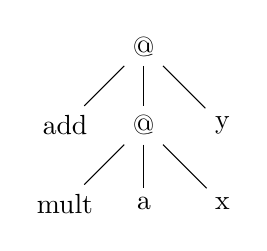
\begin{tikzpicture} 
\node (top) at (1,2) {@};
\node (plus) at (0,1) {add};
\node (mid) at (1,1) {@};
\node (y) at (2,1) {y};
\node (mult) at (0,0) {mult};
\node (a) at (1,0) {a};
\node (x) at (2,0) {x};
\draw(top) -- (plus);
\draw(top) -- (mid);
\draw(top) -- (y);
\draw(mid) -- (mult);
\draw(mid) -- (a);
\draw(mid) -- (x);
\end{tikzpicture}\vspace*{-.5em}
\end{wrapfigure}
For our purposes, symbols and applications are the most important concepts,
therefore let us fortify our intuition with the example on the right: the sum $ax+y$ above
would be represented by a tree with an application at the root, whose first child is the
symbol\footnote{Note that a symbol is not a glyph --- these are often confused, the symbol
  here stands for the mathematical concept of a sum, not the glyph $+$.} for addition, the
third child is the variable with the name $y$, and the second child is another application
whose children are the symbol for multiplication and the variables with names $a$ and $x$.

As part of the functional notation of mathematics popularized by Leibniz and Newton for
algebra, the visual appearance of a subformula was largely determined by its head
operator, which nowadays carries much of the notational conventions, which are usually
phrased in terms of the following notational characteristics of a symbol:

\begin{description}
\item[fixity (for operators):] Is the operator displayed as a prefix (like a function
  symbol), as a postfix (like the factorial symbol $!$) or as an infix (like most
  arithmetic operators)?  Operators of higher arity can also have a ``mixfix'' style;
  consider the 4-ary typing judgment operator $\Gamma\vdash_\Sigma t\colon\alpha$, which
  states that a term $t$ has type $\alpha$ in a variable context $\Gamma$ and a signature
  $\Sigma$.
\item[left and right brackets:] If an operation is bracketed, are round, square, curly,
  angle, or other brackets used? In fact brackets in mathematical vernacular are mostly
  round brackets; technical notations sometimes use others, e.g. {\mathematica} uses
  square ones throughout. Note that not all parts of a presentation that look like
  brackets are indeed. For instance in a half-open interval as $]a;b]$, is actually mixfix
  operator where the bracket-like glyphs ``$]$'' look and conventionally stretch like
  brackets, but do not match and cannot be elided like brackets. They are easy to mistake
  for brackets, since they (as all fully inhabited mixfix presentations) make brackets for
  the arguments unnecessary. We would consider it a semantic anomaly to present an
  ``interval'' operator as an infix ``;'' with obligatory left and right brackets ``$]$''
  and ``$]$''.
\item[precedence (for operators):] If an operation $O$ with a high precedence occurs as an
  argument of an operator with a lower precedence, the brackets around $O$ can be
  elided.
\item[associativity (for infix operators):] To elide brackets for $n$-ary operators
  ($n>2$), it must be known whether they are associative (i.\,e.\ $(a\circ b)\circ c =
  a\circ(b\circ c) =: a\circ b\circ c$) or obey ``left-associative'' or
  ``right-associative'' elision conventions (e.g.
  $\alpha\to\beta\to\gamma:=\alpha\to(\beta\to\gamma)$ for right-associative function
  types).
\end{description}
The first two characteristics specify the composition of the visual representations,
whereas the latter two are concerned with bracket elision. Furthermore, the {\bf{role}} of
a symbol in the formula context needs to be taken into account: Is it a simple
{\emph{constant}} like $\mathbb{R}$, a {\emph{function}} that is applied to arguments, or
a {\emph{binder}} that binds variables like $\forall x.p(x)$. This is most pronounced for
functions that can occur either applied to arguments or as the concept alone.
Presentations differ for these occasions, e.g. for the absolute value function, we write
something like $\bigl|\cdot\bigr|$ with a ``dummy argument'' $\cdot$ when it is not in an
applied context.

\subsection{Notation Definitions}\label{sec:notdef}

Mathematical formulae given in the XML-based structural formats {\openmath} and Content
{\mathml} are commonly presented by implementing one XSLT template~\cite{W3C:xslt2} per
symbol, which specifies how to transform this symbol to the output format---another XML
format like Presentation {\mathml}, or a non-XML format like {\TeX}, for example.
Appropriate templates for the arguments are usually applied recursively.

The following listing shows a straightforward way to transform the exponentiation operator
from {\openmath} to {\TeX}:
 
\begin{lstlisting}[language=XSLT,caption=An XSLT presentation template,label=lst:template]
 <xsl:template match="om:OMA[om:OMS[@cd='arith1' and @name='power']]">
   <xsl:apply-templates select="*[2]"/> <!-- first argument -->
   <xsl:text>^{</xsl:text>
   <xsl:apply-templates select="*[3]"/> <!-- second argument -->
   <xsl:text>}</xsl:text>
 </xsl:template>
\end{lstlisting}

To save authors from the tedious and error-prone task of writing similar templates for
every symbol and notation variant, different facilitations have been invented. The
probably earliest examples were the presentation architecture in
{\omdocv{1.0}}~\cite{Kohlhase:otormd00} and Naylor's\&Watt's {\openmath}
conversion~\cite{Naylor:conversion}. Both supply XML-based {\defemph{notation
    definitions}} that can be transformed into a suitable XSLT conversion style sheet by a
meta-stylesheet.

In {\omdoc}, a template like the one above would be generated from a
{\element{presentation}} element of the form
\begin{lstlisting}[mathescape]
<presentation for="power" theory="arith1" role="application" class="1">
  <style format="TeX">
    <recurse select="*[2]"/><text>^{</text><recurse select="*[3]"/><text>}</text>
  </style>
  $\ldots$
<presentation>
\end{lstlisting}
where the {\attribute[ns-elt=xsl]{match}{template}} attribute is generated from the
attributes on the {\element{presentation}} element and the contents from the ones on the
{\element{use}} element. In contrast to this, where notations definitions are thought as
directed rules from content to presentation, Naylor's\&Watt's framework views them as
equivalences between representations. For the example above we would have
\begin{lstlisting}[mathescape,language=XML,morekeywords={Notation,version,semantic-template},
caption=A Template-Based Notation Definition,label=lst:template-based]
<Notation>
  <version style="1">
    <tex>\arg{a1}{n}^{\arg{a2}{m}}</tex>
    $\ldots$
  </version>
  <semantic-template>
    <OMA><OMS cd="power" name="arith1"/>
      <OMV name="n" id="a1/>
      <OMV name="n" id="a2/>
    </OMA>
  </semantic-template>
</Notation>
\end{lstlisting}
We will call the first approach to notation specification {\defemph{symbol-based}}, as the
notation is tied to a concrete symbol, and the second one {\defemph{template-based}}. Note
that the template-based approach is in principle more directly invertible (e.g. for
parsing), and more expressive (it would e.g. allow to present $log(e,x)$ as $\ln(x)$ and
$log(b,x)$ as $\log_b(x)$). But this has not been realized in practice, since the
presentation of mathematical formulae {\emph{is indeed}} tied to symbols, so all templates
are indeed one-level like the one in the example above. On this fragment, both approaches
are equivalent. Note furthermore that many of the notational characteristics of a symbol
mentioned in section~\ref{sec:characteristics} actually do not belong to the symbol but to
its presentation. For example, the division operator, presented as $\cdot/\cdot$, has a
higher precedence than $\frac{\;\cdot\;}{\;\cdot\;}$---consider $1/(a+b)$ vs.\
$\frac{1}{a+b}$.

In {\omdocv{1.2}}~\cite{Kohlhase:omdoc1.2}, all of these characteristics can be specified
as attributes to one out of potentially multiple {\element{presentation}} elements that
refer to a {\element{symbol}}. For some aspects like mix-fixity, this declarative syntax
is not yet expressive enough; in this case, embedded XSLT templates must be used, losing
declarativity. In this paper, we rethink the notation definition system and propose a
declarative system extending ideas from the notation definition system in the {\isabelle}
theorem proving environment~\cite{Paulson:Isabelle05}.

%%% Local Variables: 
%%% mode: stex
%%% TeX-master: "presel"
%%% fill-column: 90
%%% sentence-end-double-space: nil
%%% End: 

% LocalWords:  mult xsl om OMA OMS cd arith Naylor's Watt's mathescape ns elt
% LocalWords:  tex OMV presel

 %\svnInfo $Id: features.tex 9179 2012-03-14 20:20:33Z fhorozal $
\svnKeyword $HeadURL: https://svn.omdoc.org/repos/omdoc/projects/omdoc-2.0/pragmatic-strict/features.tex $
\section{Generic Elaboration of Pragmatic Language Features}
 A \defemph{feature} consists of three components:
\begin{itemize}
  \item an {\mmt} theory, called the \defemph{feature theory},
  \item an extension of the {\mmt} grammar and type system with symbol-level declarations, called the \defemph{feature-dependent syntax},
  \item an \defemph{elaboration} of the feature-dependent syntax into {\mmt} syntax
\end{itemize}

We will abbreviate the URI \url{http://cds.omdoc.org/features} with $\cn{Feat}$.

\paragraph{Logic}
The feature of being a logic is defined as follows.
The feature theory is given by
\[\thdecl{\feath{Logic}}{\symdd{o}{}{},\;\symdd{ded}{}{}}\]
The pragmatic syntax is given by
\[Sym \;\bnfas\; \mmtaxiom{a}{F}\]
The well-formedness rule is
\[\ianc{\otermtype{\TG}{\qT}{F}{o}}
       {\osym{\TG}{\qT}{\mmtaxiom{a}{F}}}
       {}\]
\ednote{Alternatively, the semantics can be defined through elaboration. Then this would become a theorem.}

The elaboration is given by
\[\elaborate{\mmtaxiom{a}{F}}
            {\symdd{a}{\oma{ded,F}}}{}\]
\ednote{ded here actually refers to the meaning of ded within $\qT$. This must be
  discussed.}
%%% Local Variables: 
%%% mode: latex
%%% TeX-master: "paper"
%%% End: 

% LocalWords:  defemph mmt cn thdecl feath symdd symdd ded Sym bnfas mmtaxiom
% LocalWords:  ianc otermtype osym ednote

  
  
\section{MMT/OMDoc}\label{sec:mmt}
 

\begin{frame}
\frametitle{Our Core Language (strict OMDoc 2 = MMT)}
\onslide<1-2>{
\vspace{.3em}
\begin{itemize}
\item A \underline{m}odule system for \underline{m}athematical \underline{t}heories (MMT)
\vspace{.5em}
\item Foundation-independent
\vspace{.5em}
\item Logics and logical frameworks represented as theories
\vspace{.5em}
\item Generic declarative language: theories, declarations, expressions
%\begin{itemize}
%\vspace{.3em}
%\item math objects as expressions
%\vspace{.3em}
%\item symbol declarations
%\vspace{.3em}
%\end{itemize}
\end{itemize}
}
\onslide<2>{
\begin{block}{Syntax}
\begin{tabular}{llll}
Modules     &$M$      &$\bnfas$ & $\bnf{(}\theoDecl{T}{\Sigma}\bnf{)}^{\bnf{\ast}}$\\
Theories    &$\Sigma$ &$\bnfas$ & $\bnf{(}\conDeclOp[E]{c}{E} \bnfalts \lfkw{include}\;\,T\bnfalts \lfkw{meta}\;\,T\bnf{)}^{\bnf{\ast}}$\\
Expressions &$E$      &         & OpenMath expressions \\%$\bnfas$ & $x \bnfalts c \bnfalts E\,E^{\bnf{+}} \bnfalts E\,\Gamma.\,E$\\
%Contexts    &$\Gamma$ &$\bnfas$ & $\ctx{x}{E}$
\end{tabular}
\end{block}
}
\end{frame}

\begin{frame}
\frametitle{MMT Theories}
\begin{block}{Examples}
\vspace{-.3em}
%\begin{multicols}{2}
%\setlength{\columnsep}{-.5em}
\begin{columns}
\column{.4\textwidth}
\begin{twelfsig}
\tsig{\Forms}\\
$\kity$\\
$\rightarrow$\\
$\lmbd$\\
\decl{\form}{\kity}\\
\decl{\ded}{\form\to\kity}\\
\tsigend
\end{twelfsig}
\column{.5\textwidth}

\begin{twelfsig}
\tsig{\FOL}\\
\tinclude{\Forms}{}\\
\decl{\term}{\kity}\\
\decl{\wedge}{\form\to\form\to\form}\\
%\decl{\vee}{\form\to\form\to\form}\\
$\vdots$\\%\decl{\forall}{(\term\to\form)\to\form}\\
\decl{\exists}{(\term\to\form)\to\form}\\
\tsigend
\end{twelfsig}
\end{columns}
%\end{multicols}
\end{block}
\end{frame}
  
\section{A Framework for Language Extensions}\label{sec:pattern}  
 %% MATH
%\newcommand{\mathll}[2][l]{\providecommand{\nl}[1][.2cm]{\\[##1]}\begin{array}{#1}#2\end{array}}
%\newcommand{\tb}{\hspace*{.5cm}}
\newcommand{\bnf}[1]{{\color{gray}#1}}
\newcommand{\bnfas}{\bnf{::=}}
\newcommand{\bnfalt}{\bnf{|}}
\newcommand{\bnfalts}{\;\bnf{|}\;}
\newcommand{\maps}[2]{#1\mapsto #2}
\newcommand{\imorph}{\hookrightarrow}
\newcommand{\assign}[2]{#1 := #2}
\renewcommand{\maps}[2]{\assign{#1}{#2}}
\newcommand{\bnfor}[2]{(#1|#2)}
\newcommand{\dbf}{\bf}

%% For making metalevel syntax red
\newcommand{\rvdash}{\vdash}%{\mathbin{\color{red}\vdash}}
\newcommand{\rcln}{:}%{\mathbin{\color{red}:}}
\newcommand{\req}{\doteq}%{\mathbin{\color{red}=}}
\newcommand{\rleadsto}{\leadsto}%{\mathbin{\color{red}\leadsto}}

%% TYPE THEORY
\renewcommand{\arr}{\rightarrow}
\renewcommand{\P}[2]{\Pi_{#1:#2}\,}
\newcommand{\lam}[2]{\lambda_{#1:#2}\,}
\newcommand{\Terms}{Terms}
\newcommand{\Types}{Types}
\newcommand{\Sorts}{Sorts}
%\newcommand{\type}{type}
%\newcommand{\sort}{sort}
\newcommand{\varlist}{x_1:\tau_1,\ldots,x_n:\tau_n}
\newcommand{\rec}[1]{\{#1\}} % record type 
\newcommand{\lmd}[3][]{\lambda #2\ifnonempty{#1}{:#1}.\,#3}

%%LF
\newcommand{\lftype}{\mathtt{type}}
\newcommand{\lffont}[1]{\small\texttt{#1}}
\newcommand{\lfm}[1]{\mathit{#1}}
\newcommand{\kity}{\mathtt{type}}
\newcommand{\lfkind}{\mathtt{kind}}

%%Substitution, contexts, beta, eta equality
\newcommand{\beq}{\doteq_{\beta}}
\newcommand{\eeq}{\doteq_{\eta}}
\newcommand{\sub}[2]{#2 / #1}           %\sub{x}{A} means A for x
\newcommand{\subs}[2]{[#1]\,#2}         %\subs{\sub{x_1}{A_1},\sub{x_2}{A_2}}{B} means A_1 for x_1 and A_2 for x_2 in B
\newcommand{\subst}[3]{[#2 / #1]\,#3}   %\subst{x}{A}{B} means A for x in B
\newcommand{\psubst}[3]{[#2 / #1]\,#3}
\newcommand{\sappl}[2]{\hexta{#1}{#2}}
\newcommand{\ctx}[1]{\langle #1\rangle}
\newcommand{\Ctx}{\mathit{Ctx}}

%%Renaming
\newcommand{\rnm}[1]{R^{s_j}_{i.s_j}(#1)}

%% Logic Abbreviations
\newcommand{\fol}{FOL}
\newcommand{\sfol}{SFOL}
\newcommand{\dfol}{DFOL}
\newcommand{\hol}{HOL}

%% Meta-variables
\newcommand{\ptype}{\tau}  %pattern types
\newcommand{\plist}{D}     %list of declaration patterns
\newcommand{\DL}{L}        %declarative languages / logics
\newcommand{\dlm}{l}       %declarative language / logic morphisms
\newcommand{\icons}{i}     %instances                          
\newcommand{\psig}{\Theta} %pragmatic signatures
\newcommand{\psigm}{\theta} %pragmatic signatures
\newcommand{\esig}{\Phi} %elaborated signatures
\newcommand{\sfr}{\Sigma}
\newcommand{\lext}{\Sigma}

%% Declaration Patterns
%\newcommand{\pbind}[3][]{\lambda #2\ifnonempty{#1}{:#1}.\,#3}
\newcommand{\pbind}[3]{\lambda #1:#2.\,#3} %Pattern binder
\newcommand{\pappl}[2]{#1\,#2}              %Pattern application
\newcommand{\sigtp}{\texttt{Sig}}          %Type of signature fragments 
\newcommand{\match}[2]{#1\ll #2}
\newcommand{\sigfr}[1]{\{#1\}}
\newenvironment{sigfrag}{\!\left\{\!\!\!\begin{array}{l@{\,:\,}l}}{\end{array}\!\!\!\right\}}
\newcommand{\sfdecl}[3][]{#2 & #3\ifnonempty{#1}{ = #1}}
\newcommand{\qnm}[2]{\,#1\!.#2\,}

%% OpenMath Versions
\newcommand{\ombind}[1]{\beta(#1)}         %OpenMath bindings
\newcommand{\oma}[2]{{@}(#1,#2)}           %OpenMath application @(a,b,c,...,t)

%% Declarative Languages, Signatures and Morphisms
\newcommand{\dlp}[1]{D_{#1}}                                    %the set \dlp{L} of declaration patterns of language L
\newcommand{\vdecl}[2]{#1 \rcln #2}                             %variable declaratoins x : T
\newcommand{\cdecldef}[3][]{#2 \rcln #3\ifnonempty{#1}{ = #1}}     %constant declarations c : T = E for type T and definition E
\newcommand{\cdecl}[3][]{#2 \rcln #3\ifnonempty{#1}{ [= #1]}} %constant declarations c : T [= E] compact notation
\newcommand{\pdecl}[3][]{#2\ifnonempty{#1}{: #1} = #3}  %pattern declarations  p : T = P for type T and definition P
\newcommand{\pvalext}[1]{\xhookrightarrow{#1}}          %pattern-valid (legal) extensions of languages
\newcommand{\hext}[1]{\overline{#1}}                    %homomorphic extension
\newcommand{\hexta}[2]{\overline{#1}(#2)}               %homomorphic extension of a morphism applied to its argument

%% Sequences
\newcommand{\seqvar}{\varsigma}
\newcommand{\seqsubst}[3]{[#1]_{#2 / #3}}
\newcommand{\sequpto}[1]{\leq\!#1}
\newcommand{\seqind}[2]{#1_{#2}}
\newcommand{\sitem}{\iota}

%% Natural numbers
\newcommand{\add}[2]{#1 + #2}
\newcommand{\subt}[2]{#1 - #2}
\newcommand{\Nat}{\mathbb{N}}
\newcommand{\ntype}{\mathtt{Nat}}

%% Category Theory Semantics for Declaration Patterns and Translations
\newcommand{\sig}[1]{Sig^{#1}}
\newcommand{\catdl}{\mathbb{D}}
\newcommand{\Lsyn}[1][L]{#1}
\newcommand{\functh}[1][]{\mathbf{Th}\ifnonempty{#1}{(#1)}}


%% Judgments 
\newcommand{\wljudg}[1]{\rvdash #1\;\mathit{Lang}}                     %wellformed language/logic judgment
\newcommand{\wlmjudg}[3]{\rvdash #1\;\;:\;\;#2\;\rightarrow\; #3} %wellformed language/logic morphism judgment
\newcommand{\wsjudg}[2][]{\rvdash^{#1}\;#2\;\mathit{Sig}}              %wellformed signature judgment
\newcommand{\wsmjudg}[4][]{\rvdash^{#1}\;#2 \rcln #3\to #4}  %wellformed signature morphism judgment
\newcommand{\wpsjudg}[2][]{\rvdash^{#1}\;#2}             %wellformed signature judgment
\newcommand{\wpsmjudg}[4][]{\rvdash_{#1}\;#2 \rcln #3\to #4} %wellformed signature morphism judgment
\newcommand{\wesjudg}[2][]{\rvdash_{#1}\;#2}             %wellformed signature judgment
%\newcommand{\wesmjudg}[4][]{\rvdash_{#1}\;#2 \rcln #3\to #4} %wellformed signature morphism judgment
\newcommand{\wpjudg}[5][\Gamma]{#1\rvdash^{#2}_{#3} #4 \rcln #5} %wellformed pattern judgment 
\newcommand{\wejudg}[5][]{#3\rvdash^{#1}_{#2}\;#4 \rcln #5}  %wellformed expression judgment
\newcommand{\wijudg}[5][]{#3\rvdash^{#1}_{#2}\;#4 \rcln #5}  %wellformed instance judgment
\newcommand{\wcjudg}[3][]{\rvdash^{#1}_{#2}\;#3\;\mathit{Ctx}}         %wellformed context judgment
\newcommand{\wsbjudg}[4][]{#4 \rvdash_{#1}\;#2\;\rcln\;#3}   %wellformed substitution judgment
\newcommand{\pejudg}[5][\Gamma]{#1\rvdash^{#2}_{#3}\;#4 \req #5} % pattern equality judgment
\newcommand{\sejudg}[3][]{#2 \rleadsto^{#1}\;#3}         %signature elaboration judgment
\newcommand{\pmjudg}[3][\Gamma]{#1\rvdash\;#2\ll #3}     % pattern matching judgment
\newcommand{\seqjudg}[4][\Gamma]{#1\rvdash_{#2} #3 \doteq #4} % sequence equality judgment


%\newcommand{\mmtejudg}[3][]{#2\vdash^{#1} #3}         %wellformed MMT expression judgment
%\newcommand{\stjudg}[3]{#2\leadsto_{#1}#3}            %signature translation judgment
%\newcommand{\emjudg}[2]{#1\ll #2}                     %expression matches an expression
%\newcommand{\lmjudg}[3][\delta]{#1\vdash #2\ll #3}    %list of expr matches another list
%\newcommand{\ptjudg}[3][\Gamma]{#1\vdash #2 : #3}     %type judgment for patterns
%\newcommand{\etjudg}[3][\Gamma]{#1\vdash #2 : #3}     %type judgment for expressions
%\newcommand{\ltjudg}[3][\gamma]{#1\vdash #2 : #3}     %type judgment for lists

%% Rule names for judgment \wpjudg
\newcommand{\rSigFrag}{\mathit{sigFrag}}
\newcommand{\rPConst}{\mathit{const}}
\newcommand{\rPBind}{\mathit{bind}}
\newcommand{\rPAppl}{\mathit{appl}}
%\newcommand{\rpconst}{\mathit{const}}
%\newcommand{\rpctx}{\mathit{ctx}}
%\newcommand{\rpbind}{\mathit{bind}}
%\newcommand{\rpappl}{\mathit{appl}}

%% Rule names for judgment \wljudg
\newcommand{\rEDL}{\mathit{empty}}
\newcommand{\rPDL}{\mathit{pattern}}

%% Rule names for judgment \wsbjudg
\newcommand{\rEmpSub}{\mathit{empty}}
\newcommand{\rSub}{\mathit{subs}}

%% Rule names for \pejudg
\newcommand{\rPBeta}{\beta\textrm{-}\mathit{Eq}}
\newcommand{\rPEta}{\eta\textrm{-}\mathit{Eq}}

%% Rule names for \wpsjudg
\newcommand{\rAddEmpty}{\mathit{empty}}
\newcommand{\rAddInst}{\mathit{inst}}

%% Rule names for \sejudg
\newcommand{\rEmptyElab}{\mathit{empty}}
\newcommand{\rInstElab}{\mathit{inst}}


%% Old macros
%\newcommand{\matches}[3][\Gamma]{#1\vdash #2\ll #3}
%\newcommand{\lmatches}[3][\Gamma]{#1\vdash #2\ll #3}
%\newcommand{\listpat}{L}
%\newcommand{\pplist}{\pat'_1,\ldots,\pat'_{n'}}
%\newcommand{\ltype}{\mathtt{List}}
%\newcommand{\prep}[1]{\overline{#1}}
%\newcommand{\tappend}{,}
%\newcommand{\expr}{E}
%\newcommand{\etype}{\mathtt{Exp}}
%\newcommand{\lsttp}[1][]{\mathtt{List}\ifnonempty{#1}{\lbrack #1\rbrack}}
%\newcommand{\lstmap}[3]{[#3]_{#2/#1}}
%\newcommand{\lelem}[1]{#1.i}
%\newcommand{\elist}{\expr_1,\ldots,\expr_n}
%\newcommand{\dlist}{x_1:\expr_1,\ldots,x_n:\expr_n}
%\newcommand{\block}[1]{\langle #1\rangle}
%\newcommand{\typelist}{\tau_1,\ldots,\tau_n}
%\newcommand{\poftp}[1]{\widehat{#1}}
%\newcommand{\occurs}[2]{#2[#1]}
%\newcommand{\patt}{P}
%\newcommand{\pat}{P}
%\newcommand{\pcons}{c}
%\newcommand{\typelist}{\type_1,\ldots,\type_n}
%\newcommand{\oftype}[3][\Gamma]{#1 \vdash #2 : #3}
%\newcommand{\decl}[3][]{#2 : #3\ifnonempty{#1}{= #1}}
%\newcommand{\seqv}{\varsigma}
%\newcommand{\seq}{L}
%\newcommand{\stype}{\mathtt{Seq}}
%\newcommand{\ellipsis}[4][]{[#4]^{#2}_{\ifnonempty{#1}{#3 = #1}{#3 = 1}}}
%\newcommand{\sindex}[2]{#1.#2}
%\newcommand{\pSigma}{\Sigma}
%\newcommand{\psigma}{\sigma}
%\newcommand{\eSigma}{S}
%\newcommand{\esigma}{s}
%\newcommand{\lteq}{=}
%\newcommand{\dom}[1]{\mathit{dom}(#1)}    %domain
  
\section{Representing Extension Principles}\label{sec:meta}
 \svnInfo $Id: meta.tex 9199 2012-04-20 20:19:00Z frabe $
\svnKeyword $HeadURL: https://svn.omdoc.org/repos/omdoc/projects/omdoc-2.0/pragmatic-strict/meta.tex $

Formal mathematical developments can be classified based on whether they follow the
axiomatic or the definitional method. The former is common for logics where theories
declare primitive constants and axioms. The latter is common for foundations of
mathematics where a fixed theory (the foundation) is extended only by defined constants
and theorems.  In {\mmt}, both the logic and the foundation are represented as a
meta-theory $M$, and the main difference is that the definitional method does not permit
undefined constants in $M$-theories.

However, this treatment does not capture conservative extension principles:
These are meta-theorems that establish that certain extensions are acceptable even if they are not definitional.
We can understand them as intermediates between axiomatic and definitional extensions: They may be axiomatic but are essentially as safe as definitional ones. 

To make this argument precise, we use the following definition:

\begin{definition}
We call the theory family
$\Phi=\pbind{x_1}{E'_1}\ldots\pbind{x_n}{E'_n}\sigfr{\Sigma}$
\defemph{conservative} for $M$ if for every $M$-theory $T$ and all $E_1:E'_1,\ldots,E_n:E'_n$, every model of $T$ can be extended to a model of $T,\gamma(\Sigma)$, where $\gamma$ substitutes every $x_i$ with $E_i$.

  An extension declaration $\extension{e}{\Phi}$ is called \defemph{derived} if all
  constant declarations in $\Sigma$ have a definiens; otherwise, it is called \defemph{primitive}.
\end{definition}

Primitive extension declarations correspond to axiom declarations because they postulate that certain extensions of $M$ are legal. The proof that they are indeed conservative is a meta-argument that must be carried out as a part of the proof that $M$ is an adequate {\mmt} representation of the represented formalism.
Similarly, derived extension declarations correspond to theorem declarations because their conservativity follows from that of the primitive ones. More precisely:
If all primitive extension principles in $M$ are conservative, then so are all derived ones.

In the following, we will recover built-in extension statements of common representation formats as special cases of our extension declarations.
We will follow a \emph{little foundations} paradigm and state every extensions in the smallest theory in which it is meaningful. Using the {\mmt} module system, this permits maximal reuse of extension definitions. Moreover, it documents the (often implicit) foundational assumptions of each extension.

\paragraph{Implicit Definitions in {\omdoc}}
Implicit definitions of {\omdoc} 1.2 are captured using the following derived extension declaration.
If the theory $\Description$ in Figure~\ref{fig:impldef} is included into a meta-theory $M$, then $M$-theories may use implicit definitions.

\begin{figure}[ht]
\vspace{-1.5em}
\begin{center}
\begin{twelfsig}
\tsig{\Description}\\
\tmeta{\Forms}{}\\
\decl{\uexists}{(\alpha\to\form)\to\form}\\
\decl{\descr}{(\alpha\to\form)\to\alpha}\\
\decl{\descr_{\ax}}{\ded\,\uexists x\,P\,x\to \ded\,P\,(\descr\,P)}\\
[.5em]
\tpattern{\implDef}{\lflam[\kity]{\alpha}\lflam[\alpha\to\form]{P}\lflam[\ded\,\uexists x:\alpha.\,P\,x]{m}}{
 \tsfdecl{c}{\alpha\;\;=\;\;\descr\,P}\\
 \tsfdecl{c_\ax}{\ded\,\uexists x:\alpha.\,P\,x}\\
}\\
\tsigend
\end{twelfsig}
\end{center}
\vspace{-2em}
\caption{An Extension for Implicit Definitions}\label{fig:impldef}
\vspace{-1em}
\end{figure}

Note that $\Description$ requires two other connectives: A description operator ($\descr$) and a unique existential ($\uexists$) are needed to express the meaning of an implicit definition.
We deliberately assume only those two operators in order to maximize the re-usability of this theory: Using the {\mmt} module system, any logic $M$ in which these two operators are definable can import the theory $\Description$.
%In particular, we do not define the unique existential quantifier in terms of equality so that $\Description$ can be reused if $M$ does not have to have equality.

More specifically, $\Description$ introduces the definite description operator as a new
binding operator ($\descr$), and describes its meaning by the axiom $\uexists
x\,P(x)\impl\,P\,(\descr\,P)$ formulated in $\descr_{\ax}$ for any predicate $P$ on $\alpha$.
The extension $\implDef$ permits pragmatic declarations of the form $f:
\implDef\,\alpha\,P\,m$, which defines $f$ as the unique object which makes the property
$P$ valid. This leads to the well-defined condition that there is indeed such a unique
object, which is discharged by the proof $m$.  The pragmatic-to-strict translation from
Section~\ref{sec:pattern} translates the pragmatic declaration $f: \implDef\,\alpha\,P\,m$
to the strict constant declarations $f.c : \alpha = \descr\,P$ and $f.c_{\ax} :
\ded\,\uexists x:\alpha\,P\,x$.



\paragraph{Mizar-Style Functor Definitions}
The Mizar language \cite{mizar} provides a wide (but fixed) variety of special statements, most of which can be understood as conservative extension principles for first-order logic. A comprehensive list of the corresponding extension declarations can be found in \cite{IKR:mizar:11}.
We will only consider one example in Figure~\ref{fig:mizar}.


\begin{figure}[ht]
\vspace{-2em}
\begin{center}
\begin{twelfsig}
\tsig{\FunctorDefinitions}\\
\tmeta{\Forms}{}\\
\decl{\wedge}{\form\to\form\to\form}\\
\decl{\impl}{\form\to\form\to\form}\\
\decl{\forall}{(\alpha\to\form)\to\alpha}\\
\decl{\exists}{(\alpha\to\form)\to\alpha}\\
\decl{\eqn}{\alpha\to\alpha\to\form}\\
%\decl{\means}{(\alpha\to\form)\to\form}\\[.5em]
%\tpattern{\functor}{\lflam[\kity]{\alpha}\lflam[\kity]{\beta}\lflam[\alpha\to\beta\to\form]{\means}}{
% \tsfdecl{f}{\alpha\to\beta}\\
% \tsfdecl{\defthm}{\means\,x\,(f\,x)}\\
%}\\
\multicolumn{4}{@{\tb}l}{$\lfkw{extension}\;\functor\;=$}\\
& &$\lflam[\kity]{\alpha}\lflam[\kity]{\beta}\lflam[\alpha\to\beta\to\form]{\means}$\\
& &$\lflam[\ded\,\forall x:\alpha.\,\exists y:\beta.\,\means\,x\,y]{\existence}$\\
& &$\lflam[\ded\,\forall x:\alpha.\,\forall y:\beta.\,\forall y':\beta.\,\means\,x\,y\wedge \means\,x\,y'\impl y\eqn y']{\uniqueness}\,\{$\\
\multicolumn{4}{@{\tb\tb}l}{
\begin{tabular}{lll}
$\tb f$ &$:$ &$\alpha\to\beta$\\
$\tb\defthm$ & $:$ &$\ded\,\forall x:\alpha.\,\means\,x\,(f\,x)$\\
\end{tabular}}\\
&& $\}$\\
\tsigend
\end{twelfsig}
\end{center}
\vspace{-2.5em}
\caption{An Extension for Mizar-Style Functor Definitions}\label{fig:mizar}
\vspace{-1.5em}
\end{figure}

The theory $\FunctorDefinitions$ describes Mizar-style implicit definition of a unary function symbol (called a \emph{functor} in Mizar). This is different from the one above because it uses a primitive extension declaration that is well-known to be conservative. In Mizar, the axiom $\defthm$ is called the definitional theorem induced by the implicit definition. Using the extension $\functor$, one can introduce pragmatic declarations of the form $\pragmatic{c}{\functor\,A\,B\,P\,E\,U}$ that declare functors $c$ from $A$ to $B$ that are defined by the property $P$ where $E$ and $U$ discharge the induced proof obligations.

\paragraph{Flexary Extensions}
The above two examples become substantially more powerful if they are extended to implicit definitions of functions of arbitrary arity.
This is supported by our extension language by using an LF-based logical framework with term sequences and type sequences.
We omit the formal details of this framework here for simplicity and refer to \cite{Hor:patterns} instead.
We only give one example in Figure~\ref{fig:casebased} that demonstrates the potential.

\begin{figure}[ht]
\vspace{-1.5em}
\begin{center}
\begin{twelfsig}
\tsig{\CaseBased}\\
\tmeta{\Forms}{}\\
%$\wedge$\\
%$\impl$\\
%$\forall$\\
\decl{\wedge}{\form^n\to\form}\\
\decl{\vee^{!}}{\form^n\to\form}\\
\decl{\impl}{\form\to\form\to\form}\\
\decl{\forall}{(\alpha\to\form)\to\form}\\
\multicolumn{4}{@{\tb}l}{$\lfkw{extension}\;\casedef\;=\;\lflam[\mathbb{N}]{n}\lflam[\kity]{\alpha}\lflam[\kity]{\beta}\lflam[(\alpha\to\form)^n]{c}$}\\
& &$\hspace{2.65cm}\lflam[(\alpha\to\beta)^n]{d}\lflam[\ded\,\forall x:\alpha.\, \vee^{!} \lfseqbind{c_i\,x}{i}{n}]{\rho}\{$ \\
\multicolumn{4}{@{\tb\tb}l}{
\begin{tabular}{lll}
$f$ &$:$ &$\alpha\to\beta$\\
$\ax$ & $:$ &$\ded\,\forall x:\alpha.\,\wedge\,\lfseqbind{c_i\,x\,\impl\,(f\,x) = (d_i\,x)}{i}{n}$\\
\end{tabular}}\\
\multicolumn{4}{@{\tb}l}{$\}$}\\
%\tpattern{\caseBasedDef}{\lflam[\mathbb{N}]{n}\lflam[\kity]{\alpha}\lflam[\kity]{\beta}\lflam[(\alpha\to\form)^n]{c}\lflam[(\alpha\to\beta)^n]{d}\lflam[\ded\,\forall x:\alpha.\, \vee^{!} \lfseqbind{c_i\,x}{i}{n}]{m}}{
% \tsfdecl{f}{\alpha\to\beta}\\
% \tsfdecl{\ax}{\ded\,\forall x:\alpha.\,\wedge\,\lfseqbind{c_i\,x\,\impl\,(f\,x) = (d_i\,x)}{i}{n}}\\ 
%}\\
\tsigend
\end{twelfsig}
\end{center}
\vspace{-2em}
\caption{An Extension for Case-Based Definitions}\label{fig:casebased}
\vspace{-1.5em}
\end{figure}

The theory $\CaseBased$ introduces an extension that describes the case-based definition of a unary function $f$ from $\alpha$ to $\beta$ that is defined using $n$ different cases where each case is guarded by the predicate $c_i$ together with the respective definiens $d_i$.
Such a definition is well-defined if for all $x \in\alpha$ exactly one out of the $c_i\,x$ is true.
Note that these declarations use a special sequence constructor: for example, $\lfseqbind{c_i\,x}{i}{n}$ simplifies to the sequence $c_1\,x\,,\ldots,c_n\,x$.
Moreover, $\wedge$ and $\vee^!$ are flexary connectives, i.e., they take a flexible number of arguments.
In particular, $\vee^!(F_1,\ldots,F_n)$ holds if exactly one of its arguments holds.

The pragmatic declaration $\pragmatic{f}{\casedef\,n\,\alpha\,\beta\,c_1\ldots c_n\,d_1\ldots d_n\,\rho}$
%corresponds to the function definition $f(x) =\left\{
%\begin{array}{lll}
%  d_1(x) & \quad\textrm{if}\quad & c_1(x) \\
% \vdots && \vdots\\
% d_n(x) & \quad\textrm{if}\quad & c_n(x)
%\end{array}\right.
%$
corresponds to the following function definition: \[f(x) =\left\{
\begin{array}{lll}
  d_1(x) & \quad\textrm{if}\quad & c_1(x) \\
 \vdots && \vdots\\
 d_n(x) & \quad\textrm{if}\quad & c_n(x)
\end{array}\right.
\]


%In the extension $\casedef$, the unary function $f$ is defined using $n$ different cases guarded by the predicates $c_i$ together with the respective definientia $d_i$. 
%Here, $(\alpha\to\form)^$ denotes the sequence of types $\alpha\to\form$ of length $n$.


%\multirow{3}{*}{Immediate} & RR & Round Robin \\
%\[
%f(x) =
%\begin{cases}
% D_1, & \text{if } C_1 \text{ is even} \\
% D_2, & \text{if } C_2 \text{ is odd}
%\end{cases}
%\]


\paragraph{HOL-Style Type Definitions}
Due to the presence of $\lambda$-abstraction and a description operator in HOL \cite{churchtypes}, a lot of common extension principles become derivable in HOL, in particular, implicit definitions.

But there is one primitive definition principle that is commonly accepted in HOL-based formalizations of the definitional method: A Gordon/HOL type definition \cite{hol} introduces a new type that is axiomatized to be isomorphic to a subtype of an existing type. This cannot be expressed as a derivable extension because HOL does not use subtyping.


\begin{figure}[ht]
\vspace{-1.5em}
\begin{center}
\begin{twelfsig}
\tsig{\Types}\\
\tmeta{\Forms}{}\\
\decl{\forall}{(\alpha\to\form)\to\form}\\
\decl{\exists}{(\alpha\to\form)\to\form}\\
\decl{\doteq}{(\alpha\to\alpha)\to\form}\\
\tpattern{\typeDef}{\lflam[\kity]{\alpha}\lflam[\alpha\to\form]{A}\lflam[\ded\,\exists x:\alpha.\,A\,x]{P}}{
 \tsfdecl{T}{\kity}\\
 \tsfdecl{\Rep}{T\to\alpha}\\
 \tsfdecl{\Abs}{\alpha\to T}\\
 \tsfdecl{{\Rep'}}{\ded\,\forall x:T.\,A\,(\Rep\,x)}\\
 \tsfdecl{{\RepInv}}{\ded\,\forall x:T.\,\Abs\,(\Rep\,x) \doteq x}\\
 \tsfdecl{{\AbsInv}}{\ded\,\forall x:\alpha.\,A\,x\impl\Rep\,(\Abs\,x) \doteq x}\\
}\\
\tsigend
\end{twelfsig}
\vspace{-1.5em}
\caption{An Extension for HOL-Style Type Definitions}\label{fig:typedef}
\end{center}
\vspace{-1.5em}
\end{figure}

The theory $\Types$ in Figure~\ref{fig:typedef}, formalizes this extension principle. Our symbol names follow the implementation of this definition principle in Isabelle/HOL \cite{isabellehol}.
%, which takes a type $\alpha$, a predicate $A$ on $\alpha$ and a proof that $A$ is non-empty and  
Pragmatic declarations of the form $\pragmatic{t}{\typeDef\,\alpha\,A\,P}$ introduce a new non-empty type $t$ isomorphic to the predicate $A$ over $\alpha$. Since all HOL-types must be non-empty, a proof $P$ of the non-emptiness of $A$ must be supplied. 
More precisely, it is translated to the following strict constant declarations:
\begin{itemize}
\item $t.T: \kity$ is the new type that is being defined,
\item $t.\Rep: t.T\to\alpha$ is an injection from the new type $t.T$ to $\alpha$,
\item $t.\Abs:\alpha\to t.T$ is the inverse of $t.\Rep$ from $\alpha$ to the new type $t.T$,
\item $t.\Rep'$ states that the property $A$ holds for any term of type $t.T$,
\item $t.\RepInv$ states that the injection of any element of type $t.T$ to $\alpha$ and back is equal to itself,
\item $t.\AbsInv$ states that if an element satisfies $A$, then injecting it to $t.T$ and back is equal to itself.
\end{itemize}

HOL-based proof assistants implement the type definition principle as a built-in statement.
They also often provide further built-in statements for other definition principles that become derivable in the presence of type definitions, e.g., a definition principle for record types.
For example, in Isabelle/HOL \cite{isabellehol}, HOL is formalized in the Pure logic underlying the logical framework Isabelle \cite{isabelle}.
But because the type definition principle is not expressible in Pure, it is implemented as a primitive Isabelle feature that is only active in Isabelle/HOL.

%For all $x$, $f(x)$ is the unique $y$ such that $p(x,f(x))$.

%%% Local Variables: 
%%% mode: latex
%%% TeX-master: "paper"
%%% End: 

% LocalWords:  wrapfigure vspace twelfsig tsig kity ded ineq tpattern lflam thm
% LocalWords:  tsfdecl tsfdecldef tsigend ednote ptos impldef texttt forall lst
% LocalWords:  p2srule lstlisting mathescape expfun omdoc bigl desctheory impl
% LocalWords:  uexists lfseqbind tm tp tpj fhorozal newpart mmt pbind ldots
% LocalWords:  sigfr defemph tmeta descr doteq defthm Flexary casebased lfkw
% LocalWords:  casedef mathbb hspace noindent multirow Bigg textrm vdots RepInv
% LocalWords:  churchtypes AbsInv isabellehol

  
\section{Syntax Extensions and Surface Languages}\label{sec:syntax}
\svnInfo $Id: syntax.tex 9195 2012-04-20 12:26:50Z frabe $
\svnKeyword $HeadURL: https://svn.omdoc.org/repos/omdoc/projects/omdoc-2.0/pragmatic-strict/syntax.tex $

Our definitions from Section~\ref{sec:pattern} permit pragmatic \emph{abstract} syntax,
which is elaborated into strict abstract syntax.  For human-oriented representations, it
is desirable to complement this with similar extensions of pragmatic \emph{concrete}
syntax.  While the pragmatic-to-strict translation at the abstract syntax level is usually
non-trivial and therefore not invertible, the corresponding translation at the concrete
syntax level should be compositional and bidirectional.

\subsection{\protect\omdoc Concrete Syntax for EL Declarations}\label{sec:omdoc-concrete}

First we extend {\omdoc} with concrete syntax that exactly mirrors the abstract syntax
from Section~\ref{sec:pattern}. The declaration $\extension{e}{\lambda x_1:E_1.\,\ldots\lambda x_n:E_n.\,\{\Sigma\}}$
is written as
\begin{lstlisting}[mathescape,morekeywords={extension,parameter}]
<extension name="$e$">
  <parameter name="$x_1$">$\om{E_1}$</parameter>
  $\hspace{1cm}\vdots$
  <parameter name="$x_n$">$\om{E_n}$</parameter>
  <theory>
  $\hspace{.45cm}\om{\Sigma}$
  </theory>
</extension>
\end{lstlisting}
Here we use the box notation $\om{A}$ to gloss the XML representation of an entity $A$ given in abstract syntax.

Similarly, the pragmatic declaration $\pragmatic{c}{e\,E_1\ldots E_n}$ is written as

\begin{lstlisting}[mathescape,morekeywords={pragmatic}]
<pragmatic name="$c$" extension="$\llquote{M}?e$">
  $\om{E_1}\ldots\om{E_n}$
</pragmatic>
\end{lstlisting}
Here $\llquote{M}$ is the meta-theory in which $e$ is declared so that $\llquote{M}?e$ is the {\mmt} URI of the extension.

\begin{example}
  For the implicit definitions discussed in Section~\ref{sec:pattern}, we use the extension
  $\implDef$ from Figure~\ref{fig:impldef}, which we assume has namespace URI \llquote{U}.
  If $\rho$ is a proof of unique existence for an $f$ such that $f'=f\wedge f(0)=1$, then the exponential function is defined in XML by

\begin{lstlisting}[mathescape,label=lst:expdef,morekeywords={pragmatic}]
<pragmatic name="exp" extension="$\mmturi{\llquote{U}}\Description\implDef$">
  $\om{\lambda f.f'=f\wedge f(0)=1}$  $\om{\rho}$
</pragmatic>
\end{lstlisting}
\end{example}

\subsection{Pragmatic Surface Syntax}

\omdoc is mainly a machine-oriented interoperability format, which is not intended for
human consumption. Therefore, the EL-isomorphic syntax introduced is sufficient in
principle -- at least for the formal subset of \omdoc we have discussed so far.

\omdoc is largely written in the form of ``surface languages'' -- domain-specific
languages that can be written effectively and transformed to \omdoc in an automated
process. For the formal subset of \omdoc, we use a \mmt-inspired superset of the
Twelf/LF~\cite{twelf,lf} syntax, and for informal \omdoc we use
\sTeX~\cite{Kohlhase:ulsmf08}, a semantic extension of {\TeX/\LaTeX}. 

For many
purposes like learning the surface language or styling \omdoc documents,
\defemph{pragmatic surface syntax}, i.e., a surface syntax that is closer to the
notational conventions of the respective domain, has great practical advantages.
It is possible to support, i.e., generate and parse, pragmatic surface
syntax by using the macro/scripting framework associated with most representation
formats.

For instance, we can regain the XML syntax familiar from \omdoc1.2
via notation definitions that transform between \lstinline|pragmatic| elements and the
corresponding {\omdoc} 1.2 syntax. For Twelf/LF, we would extend the module system preprocessor, and for Isabelle we would extend the
SML-based syntax/parsing subsystem. We have also extended \sTeX as an example of a
semi-formal surface language. Here we used the
macro facility of {\TeX} as the computational engine. We conjecture that most practical
surface languages for MKM can be extended similarly.

These translations proceed in two step. Firstly, pragmatic surface syntax is translated into our pragmatic {\mmt} syntax. Our language is designed to make this step trivial: in particular, it does not have to look into the parameters used in a pragmatic surface declaration.
Secondly, pragmatic {\mmt} syntax is type-checked and, if desired, translated into strict {\mmt} syntax.
All potentially difficult semantic analysis is part of this second step.
This design makes it very easy for users to introduce their own pragmatic surface syntax.

%%% Local Variables: 
%%% mode: latex
%%% TeX-master: "paper"
%%% End: 

% LocalWords:  omdoc ednote lstlisting mathescape llquote llquote llqn ldots cn
% LocalWords:  llqn mmt frabe newpart emph implDef impldef lst expdef exu-proof
% LocalWords:  footnotemark exp footnotetext expr exunique exu stex hspace lf
% LocalWords:  morekeywords vdots mmturi ulsmf08 defemph

 
\section{Conclusion \& Future Work}\label{sec:concl}
 \section{Conclusion and Further Work}\label{sec:conclusion}

We have demonstrated that a Markup Language for the {\emph{content}} of physics can be
designed by extending the content and context markup format {\omdoc} with a
representational infrastructure for the principal objects of physics: observables,
systems, and experiments. The resulting language {\physml} is able to catch the logical
and operational structure specific to physics, differentiating this field from others. The
extension presented in this paper is part of the ongoing enterprise to extend the {\omdoc}
format to the {\bf{STEM}} fields ({\underline{S}}ciences, {\underline{T}}echnology,
{\underline{E}}ngineering and {\underline{M}}athematics).


The next step is now to evaluate the language by marking up a larger body of knowledge in
physics in {\physml}.  We have started work on the technically ubiquitous and basic field
of thermostatics. This should give us a clear indication whether {\physml} is adequate for
all of physics, or pinpoint the necessary changes to the language design.  An
international collaboration on the further development of {\physml} is looked for,
including experts from theoretical and applied physics and related fields, in particular
mathematics and chemistry.

New and powerful services can be implemented once the scientific content can be
semantically encoded, retrieved, and reused digitally.  In physics, these include the
search for other experiments on the same observables, dimension and algebraic checking of
mathematical equations, mapping to other mathematical representations of the same
theoretical physical expression, etc.

Using the approach of analyzing the operational and logical practices of a scientific
discipline field, and map this to field-specific modules extending the semantic markup
language {\omdoc} will allow to spread semantic content markup to other scientific fields.

With authors to increasingly make use of markup languages, and retrieval engines
following suit to offer intelligent search algorithms making use of the known markup
languages, users will gain effective tools to increase the reachout of their scientific work,
having the {\emph{content}}, not just the text, of the work of others at their fingertips.

%%% Local Variables: 
%%% mode: LaTeX
%%% TeX-master: "mkm06"
%%% End: 

% LocalWords:  mkm


\bibliographystyle{alpha}
\bibliography{bib/historical,bib/systems,bib/rabe,bib/pub_rabe,bib/kwarc,local}
%\newpage
%\begin{appendix}
%  \svnInfo $Id: csyntax.tex 9195 2012-04-20 12:26:50Z frabe $
\svnKeyword $HeadURL: https://svn.omdoc.org/repos/omdoc/projects/omdoc-2.0/pragmatic-strict/csyntax.tex $

\section{Pragmatic {\omdoc} Syntax}\label{sec:omdoc-pragmatic}

For implicit definitions we have the notation definition in listing~\ref{lst:notation}
(slightly simplified elemental XML notation). Recall from~\cite{KMR:presentation:08} that notation
definitions are essentially transformation rules that use named \lstinline|expr| elements
as variables in the heads and \lstinline|render| for the recursive calls of the
transformation.
\begin{lstlisting}[mathescape,label=lst:notation,morekeywords={pragmatic},
  caption=A Notation Definition for implicit Definitions]
<notation format="OMDoc-pragmatic">
  <prototype>
    <pragmatic name="$c$" extension="$\mmturi{\llquote{V}}\Description\implDef$">
      <expr name="prop"/>
      <expr name="proof"/>
    </pragmatic>
  </prototype>
  <rendering> 
   <definition type="implicit" name="$c$" exunique="$c.\exu$">
      <render name="prop"/>   
    </definition>
    <assertion name="$c.\exu$" type="theorem">
       <OMA>
          <OMS cd="$\Description$" name="\implDef"/>
          <render name="prop"/>
        </OMA>
    </assertion>
    <proof for="$c.\exu$"><render name="proof"/></proof>
  <rendering>
</notation>
\end{lstlisting}
Note that the ``direction'' of the notation definition may be confusing at first. But it
becomes natural: Here the \omdoc1.2 syntax can be regarded as a surface language into
which the \lstinline{statement} elements are presented into. But note that the notation
definitions can also be ``turned around'' for parsing. We are currently working on parsing
technology that integrates this idea.

\section{Pragmatic Concrete Syntax in \protect\sTeX}\label{sec:stex-pragmatic}
\lstset{language={[sTeX]TeX},morekeywords={extkey,extension}}

Now we show how to extend one of the {\omdoc} surface languages (formats intended for
human authoring and transformation to OMDoc) with pragmatic concrete syntax. We have
extended the \sTeX format~\cite{Kohlhase:ulsmf08} with an extension language, which we
present here as an example how the ideas presented in this paper can be extended to
semi-formal MKM formats. The next listing shows the extensions for implicit definitions.
The \lstinline|\extension| macro takes the name of the extension as a first required
argument and then uses the second and third arguments to define an environment of that
name in the usual way. The main problem in {\TeX}-based formats is argument passing; in
our extension language we use two ways. ``Small'' arguments are passed as key/value pairs;
we use the \lstinline|\extkey| macro to declare keys. ``Large'' arguments are naturally
packaged in environments of their own which are declared as ``continuations'' by the
\lstinline|cont| key in the optional argument of \lstinline|extension|. 

\begin{lstlisting}[caption=Extending \protect\sTeX by Implicit Definitions]
\begin{module}[id=ImplicitDefinitions]
\ldots
\extkey{idef}{name}
\extkey{idef}{title}
\extension{idef}
{\begin{def}[\namarg{idef}{title}]\label{idef.\namarg{idef}{name}}}
{\end{def}}
\extkey{exu}{for}
\extension[cont=idef]{exu}
{\begin{thm}[Existence and Uniqueness for \ref{\namarg{exu}{for}}]
\label{\namarg{exu}{for}.exu}}
{\end{thm}}
\extkey{exup}{for}
\extension[cont=idef]{exup}
{\begin{proof} (for \ref{\namarg{exu}})}
{\end{proof}}
\end{module}
\end{lstlisting}
Note the structural similarity of these extension declarations to the
\lstinline[language={[1.3]OMDoc}]|rendering| element in
Listing~\ref{lst:notation}.
Given this we can use the three induced environments
once we have imported the module above. 

\begin{lstlisting}[language={[sTeX]TeX},morekeywords={extkey,extension}]
\importmodule{ImplicitDefinitions}
\begin{idef}[name=exp,title=Exponential Function]
  The exponential function is that function $f$ with $f'=f$ and $f(0)=1$.
\end{idef}
\begin{exu}[for=exp]
  There is exactly one function $f$ with with $f'=f$ and $f(0)=1$.
\end{exu}
\begin{exup}[for=exp]
  \ldots
\end{exup}
\end{lstlisting}
Note that the OMDoc generated from the \sTeX can either be in the pragmatic concrete syntax from
Section~\ref{sec:omdoc-pragmatic} or directly in the concrete syntax from
Section~\ref{sec:omdoc-concrete}.


%%% Local Variables: 
%%% mode: latex
%%% TeX-master: "paper"
%%% End: 

% LocalWords:  csyntax.tex omdoc omdoc-pragmatic lst expr lstlisting mathescape
% LocalWords:  morekeywords mmturi llquote implDef exunique exu stex-pragmatic
% LocalWords:  lstset extkey ulsmf08 cont ldots idef namarg namarg thm exup exp

%\end{appendix}
\end{document}

% LocalWords:  maketitle pn pnp pns printbibliography prel ednote foo concl mmt
%%% Local Variables: 
%%% mode: latex
%%% TeX-master: "paper"
%%% End: 
% LocalWords:  omdoc newpage csyntax
